% !TEX encoding = UTF-8 Unicode
\documentclass[14pt]{extarticle}

\usepackage{color}
\usepackage{url}
\usepackage[T2A]{fontenc} % enable Cyrillic fonts
\usepackage[utf8]{inputenc} % make weird characters work
\usepackage{graphicx}

\usepackage[english,serbian]{babel}
%\usepackage[english,serbianc]{babel} %ukljuciti babel sa ovim opcijama, umesto gornjim, ukoliko se koristi cirilica

\usepackage[unicode]{hyperref}
\hypersetup{colorlinks,citecolor=green,filecolor=green,linkcolor=blue,urlcolor=blue, basicstyle=small}

\usepackage{listings}

%\newtheorem{primer}{Пример}[section] %ćirilični primer
\newtheorem{primer}{Primer}[section]

\definecolor{mygreen}{rgb}{0,0.6,0}
\definecolor{mygray}{rgb}{0.5,0.5,0.5}
\definecolor{mymauve}{rgb}{0.58,0,0.82}

\fontsize{40}{48}
\lstset{ 
  backgroundcolor=\color{white},   % choose the background color; you must add \usepackage{color} or \usepackage{xcolor}; should come as last argument
  basicstyle=\small\ttfamily,        % the size of the fonts that are used for the code
  breakatwhitespace=false,         % sets if automatic breaks should only happen at whitespace
  breaklines=true,                 % sets automatic line breaking
  captionpos=b,                    % sets the caption-position to bottom
  commentstyle=\color{mygreen},    % comment style
  deletekeywords={...},            % if you want to delete keywords from the given language
  escapeinside={\%*}{*)},          % if you want to add LaTeX within your code
  extendedchars=true,              % lets you use non-ASCII characters; for 8-bits encodings only, does not work with UTF-8
  firstnumber=0,                % start line enumeration with line 1000
  frame=single,	                   % adds a frame around the code
  keepspaces=true,                 % keeps spaces in text, useful for keeping indentation of code (possibly needs columns=flexible)
  keywordstyle=\color{blue},       % keyword style
  language=Python,                 % the language of the code
  morekeywords={*,...},            % if you want to add more keywords to the set
  numbers=left,                    % where to put the line-numbers; possible values are (none, left, right)
  numbersep=5pt,                   % how far the line-numbers are from the code
  numberstyle=\tiny\color{mygray}, % the style that is used for the line-numbers
  rulecolor=\color{black},         % if not set, the frame-color may be changed on line-breaks within not-black text (e.g. comments (green here))
  showspaces=false,                % show spaces everywhere adding particular underscores; it overrides 'showstringspaces'
  showstringspaces=false,          % underline spaces within strings only
  showtabs=false,                  % show tabs within strings adding particular underscores
  stepnumber=2,                    % the step between two line-numbers. If it's 1, each line will be numbered
  stringstyle=\color{mymauve},     % string literal style
  tabsize=2,	                   % sets default tabsize to 2 spaces
  title=\lstname                   % show the filename of files included with \lstinputlisting; also try caption instead of title
}

\begin{document}

\title{Klasifikacija HCC ćelija\\ \small{Seminarski rad u okviru kursa Istraživanje podataka 2}}

\author{Jovana Nikolić\\ \small{jovananiki7@gmail.com}}


\maketitle


\tableofcontents

\newpage

\section{Uvod}
\label{sec:uvod}
Istraživanje podataka je sve prisutnija oblast u raznim naukama. Usled velikog priliva podataka neophodno je bilo razviti algoritme koji u prihvatljivom vremenu obrađuje date podatke. Samo neke od oblasti gde se primenjuje su medicina, biologija, statistika, veštačka inteligencija...

U ovom seminarskom radu biće predstavljen detaljan opis postupka klasifikacije ćelija i prikazani rezultati iste. Pre pocetka i primene algoritama potrebno je upoznati se samim podacima sto je opisano u prvom delu. Tema predprocesiranja je opisana u narednom poglavlju, dok su algoritmi klasifikacije i rezultati glavna tema ovog rada. Na samom kraju izvršena je analiza dobijenih rezultata. Za sve primenjene postupke koričćen je programski jezik Python3. Uz standardnu biblioteku koju nudi Python upotrebljivane su još i biblioteke panda, numpy, sklearn i matplotlib (Listing 1)

\begin{lstlisting}[caption={Import biblioteka},frame=single, label=simple]
import numpy as np
import pandas as pd
import matplotlib.pyplot as plt
from mpl_toolkits.mplot3d import Axes3D
from sklearn.decomposition import PCA
from sklearn.preprocessing import StandardScaler
\end{lstlisting}


\section{Skup podataka} 
Podaci koji se klasifikuju su dobijeni iz perifernih mononuklearnih krvnih ćelija (Peripheral blood mononuclear cells, PBMCs) PBMC tipa HCC. Ove celije se koriste u istraživanju u različitim oblastima biomedicine, poput infektivnih bolesti, imunologije,
maligniteta, razvoja vakcina i slično. Glavna funkcija PBMC ćelija je imuna odbrana organizma. Svaki tip ćelije ima karakteristicne obrasce ('mustre') proteina i gena koje ih međusobno razlikuju i mogu da se koriste za podelu prema njihovom tipu.

 Sama struktura podaka nad kojima se vrše analize se sastoje od tri zasebna .csv fajla. Svaki fajl predstavlja matricu podataka gde prvi red sadrži redni broj ćelije koja je ispitivana, a prva kolona identifikaciju gena. Vrednosti u matrici sadrže broj transkripta gena  u ćeliji. Takodje svaka datoteka predstavlja jednu klasu. Na Slici 1 dat je isečak iz date matrice zbog sticanja uvida o izgledu samih fajlova.
 
\begin{figure}[h!]
\begin{center}
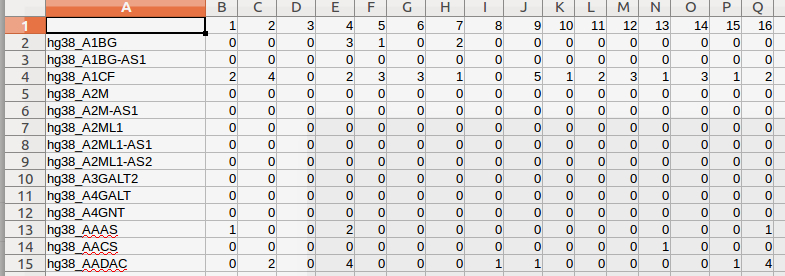
\includegraphics[scale=1.5]{slika1.jpg}
\end{center}
\caption{Fajl za obradu}
\label{fig:pande}
\end{figure}

Radi lakšeg snalaženja dati fajlove imenujemo sa HCC01.csv, HCC02.csv i HCC03.csv. U Tabeli 1 mogu se videti poređenja veličine i broja kolona sva tri fajla, dok svi fajlovi imaju 31221 red.

\begin{table}[h!]
\begin{center}
\caption{ Poređenja velicina fajlova }
\begin{tabular}{|c|c|c|} \hline
naziv& broj kolona&  velicina\\ \hline
HCC01.csv& 895 &56.5MB\\ \hline
HCC02.csv&2083 &131.1MB\\ \hline
HCC03.csv&684 &42.1MB\\ \hline\end{tabular}
\label{tab:tabela1}
\end{center}
\end{table}



Na samom početku učitavamo podatke korišćenjem funkcije pd.read\_csv. Kada su podaci učitani mozemo započeti analizu, obradu i klasifikaciju datih podataka što sledi u nastavku.

\section{Predprocesiranje}	
\label{sec:termini_i_citiranje}

Nakon što smo se upoznali sa podacima i učitali date fajlove u ovom poglavlju opisaćemo procees predprocesiranja. Struktura podataka je takva da postoji primetno veliki broj redova koji sadrže isključivo nule, ili samo jednu vrednost različitu od nule. Takvi redovi nemaju značaj za klasifikaciju tako da ćemo ih eliminisati. Programski kod kojim smo ovo postigli je prikazan u nastavku (Listing 2).

\begin{lstlisting}[caption={Redukcija redova},frame=single, label=simple]
tabela1.drop(tabela1.columns[[0]], axis=1, inplace=True)
tabela10 = tabela1[(tabela1.T != 0).any()]
i=1
j=0
brojac=0
for i in range(1, redovi):
	if brojac==1:
		tabela10.drop(tabela10.index[i])
	for j in range(0,kolone):
		if tabela10.iloc[i,j]!=0:
			brojac=brojac+1
		if brojac>1:
			brojac=0
			break			
redovi = tabela10.shape[0]  
kolone = tabela10.shape[1]
print(redovi,kolone)  
\end{lstlisting}

Radi smanjenja vremena izvršavanja, nad svakim fajlom posebno je primenjen ovaj postupak i u nastavku će biti učitani novonastali fajlovi. U Tabeli 2 prikazana je odnos broja redova pre i posle uklanjanja nepotrebnih instanci.

\begin{table}[h!]
\begin{center}
\caption{ Broj redova pre i nakon uklanjanja 0 redova}
\begin{tabular}{|c|c|c|} \hline
naziv& ukupan broj redova&  broj redova bez 0 redova\\ \hline
HCC01.csv& 31221 &15584\\ \hline
HCC02.csv&31221&18093\\ \hline
HCC03.csv&31221 &14085\\ \hline\end{tabular}
\label{tab:tabela1}
\end{center}
\end{table}

Sledeći korak pre same klasifikacije jeste spajanje tabela. Međutim, želimo da imamo i vizuelizaciju podataka za svaku klasu. Da bi smo to izvrsili potrebno je normalizovati podatke. Nakon toga izvršen je PCA(Principal component analysis) algoritam kojima je smanjena dimenzionalnost matrice na 3 dimenzije da bi mogli prikazati podatke na 3D dijagramu. Ovi koraci prikazani su u Listingu 3.

\begin{lstlisting}[caption={Normalizacija i PCA},frame=single, label=simple]
x = tabela10.values
standard_scaler = StandardScaler()
x_standardized = standard_scaler.fit_transform(x)
tabela10=pd.DataFrame(x_standardized, index=tabela10.index.values)

pca = PCA(3)
x = tabela10.values
x = pca.fit_transform(x)
tabela10=pd.DataFrame(x, index=tabela10.index.values)
tabela10.to_csv("fajl3.csv", encoding='utf-8', index=False)

\end{lstlisting}

Dimenzionom redukciom dobili smo padatke koje je moguće predsaviti na 3D dijagramima (Slika 2) koji su generisani propratnim kodom (Listing 4). Moze se primetiti da su geni iz jedne klase grupisani oko jednog polja dijagrama. 

\begin{lstlisting}[caption={Vizuelizacija},frame=single, label=simple]
fig = plt.figure()
ax = fig.add_subplot(111, projection='3d')
ax.scatter(x[:, 0], x[:, 1], x[:, 2])
plt.show()

\end{lstlisting}
\begin{figure}[h!]
\begin{center}
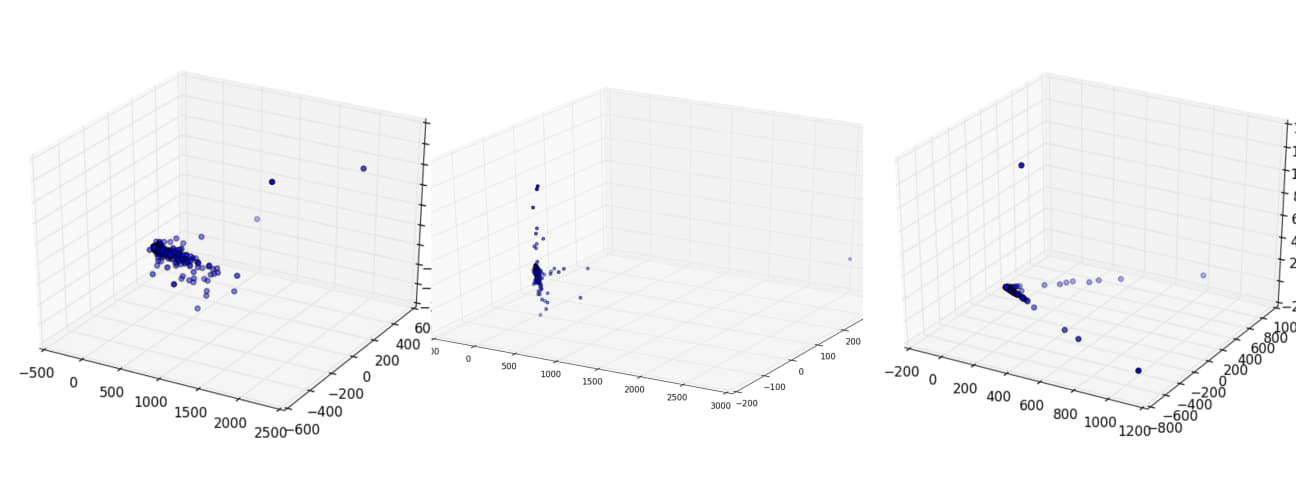
\includegraphics[scale=0.25]{slika2.jpg}
\end{center}
\caption{3D plot}
\label{fig:pande}
\end{figure}

Konačno prelazimo na spajanje naših fajlova u jedan fajl. Funkcije kojima smo ovo postigli su navedene u Listingu 4. Nakon učitavanja fajlova, svaki fajl je transponovan, uklonjene su 0 kolone i dodata mu je numerička oznaka klase, a zatim je spojen u jedan fajl nad kojim je vršen proces klasifikacije u nastavku ovog rada. 

\begin{lstlisting}[caption={Spajanje},frame=single, label=simple]

import pandas as pd
import numpy as np
import gc

#citanje fajlova
fajl1=pd.read_csv("007_HCC_cells_csv.csv", index_col = False)
fajl2=pd.read_csv("008_HCC_cells_csv.csv", index_col = False)
fajl3=pd.read_csv("009_HCC_cells_csv.csv", index_col = False)

#transponovanje i brisanje prve kolone koja oznacava redni broj
fajl1 = fajl1.T
kolone1 = fajl1.iloc[0, :]
fajl1 = fajl1.iloc[1:, :]
fajl1.columns = kolone1
gc.collect()

fajl2 = fajl2.T
kolone2 = fajl2.iloc[0, :]
fajl2 = fajl2.iloc[1:, :]
fajl2.columns = kolone2
gc.collect()

fajl3 = fajl3.T
kolone3 = fajl3.iloc[0, :]
fajl3 = fajl3.iloc[1:, :]
fajl3.columns = kolone3
gc.collect()

#dodeljivanje klase
fajl1['class'] = 0
fajl2['class'] = 1
fajl3['class'] = 2
gc.collect()

#spajanje i brisanje nula kolona
spojeni = pd.concat([fajl1,fajl2,fajl3], axis = 0, ignore_index = True)
spojeni.loc[:, (spojeni != 0).any(axis=0)]
spojeni.to_csv('./spojeni.csv', index = False)
  

\end{lstlisting}






\section{Proces klasifikacije}
\label{Klasifikacija}

Nakon što smo podatke sredili i doveli u oblik pogodan za klasifikaciju prelazimo na primenu raznih oblika klasifikacije. Naš cilj je da na osnovu dobijenih podataka utvrdimo zakonitosti i na osnovu njih istreniramo naš model za što bolju klasifikaciju. Biće primenjene metode K najbližih suseda, SVM algoritam, Drveta odlučivanja, Bajesov algoritam i neuronske mreže. U poglavlju koje sledi za svaku vrstu klasifikacije biće menjani parametri i prikazivani rezultati. Pre primene određenog postupka potrebno je da skup podataka podelimo na trening i test skup.Podela je izvršena tako da trening skup sadrži 70\% početnih podataka. Zatim su nad trening podacima sprovedeni navedeni algoritmi i dobijeni određeni zaključi pomoću test skupa. Funkcije kojima smo ovo postigli i zatim kao početni primer primenili K najbližih suseda su prikazane u Listingu 6. 

\begin{lstlisting}[caption={Klasifikacija},frame=single, label=simple]

    #citanje podataka
    df = pd.read_csv('./tabela.csv')
    #X skup na osnovu koga klasifikujemp
    X = df.loc[:, df.columns != 'class']
    #y skup vrednosti koji oznacavaju klasu
    y = df[['class']]

    #podela na test i trening skup
    X_train, X_test, y_train, y_test = train_test_split(X, y, test_size=0.3)

    #clf menjamo u zavisnosti od metode koju koristimo
    #u nastavku rada su navedeni svi pozivi funkcija koje smo koristili
    clf = KNeighborsClassifier(n_neighbors=5, weights='distance')
    clf.fit(X_train, y_train.values.ravel())
    
    #vrsimo predikciju
    y_test_predicted = clf.predict(X_test)
    y_train_predicted = clf.predict(X_train)
    
    #racunamo rezultate
    train_acc = clf.score(X_train, y_train)
    test_acc = clf.score(X_test, y_test)
    train_conf = sklearn.metrics.confusion_matrix(y_train, y_train_predicted)
    test_conf = sklearn.metrics.confusion_matrix(y_test, y_test_predicted)  
    
    #stampanje
    print('Preciznost trening skupa: {}'.format(train_acc))
    print("Matrica konfuzije:\n{}".format(train_conf))
    print('Preciznost test skupa: {}'.format(test_acc))
    print("Matrica konfuzije:\n{}".format(test_conf))


\end{lstlisting}

\section{Rezultati}
\label{Rezultati}
Rezultate prikazujemo za svaki od algoritama u vidu matrica konfuzije i preciznosti. Ako je preciznost 1 naš model nije dobar jer dolazi do preprilagodjavanja što govori da se model previše oslanja na podatke iz trening skupa. Mala preciznost takođe govori da je model loš. Podrazumevano je da čitalac poseduje predznanje vezano za korišcene metode tako da principi rada algoritama nisu detaljno opisivani.

\subsection{K najbližih suseda}
\label{subsec:podnaslovM}
Ovaj algoritam se zasniva na nalaženju najbližih suseda u svakoj iteraciji za svaki podatak. Kao parametari zadaje se vrednost k koja govori koliko suseda uzimamo u obzir. Veća vrednost parametra je pogodnija za rad sa šumovima. Kao mera rastojanja najčesće se koristi Euklidsko rastojanje ali se mogu koristiti i druge metrike za zadavanje težine čvorova poput uniforme težine. Parametri se zadaju u pozivu funkicje prikazanom u Listingu 7. 

\begin{lstlisting}[caption={Vizuelizacija},frame=single, label=simple]

clf =  KNeighborsClassifier(n_neighbors=3, weights='uniform')
clf =  KNeighborsClassifier(n_neighbors=10, weights='uniform')

clf =  KNeighborsClassifier(n_neighbors=3, weights='distance')
clf =  KNeighborsClassifier(n_neighbors=10, weights='distance')

\end{lstlisting}

Listing 8 prikazuje izlaze iz programa sa različitim vrednostima parametara koji su menjani zarad dobijanja boljeg modela. Za vrdnost k testirana je vrednost 3 i 10, dok je za metriku birano Euklidsko rastojanje i unifomna dodela težina. Iz rezultata se vidi da uniformna raspodela tezina daje ne tako dobar model sa nedovoljno dobrom preciznosti i za trening i za test skup, gde je npr za drugu klasu pogrešno klasifikovao skoro petinu instanci. Ako se posmatra distanca situacija se menja i za trening skup dolazi do dobrog klasifikovanja celog skupa dok je za test skup preciznost jako blizu jedinici. Sa porastom vrednosti k dobijamo lošije modele za uniformnu raspodelu dok se za rastojanje situacija znatno ne menja.

\begin{lstlisting}[caption={Vizuelizacija},frame=single, label=simple]

**knn 3 uniform**
Preciznost trening skupa: 0.88259
Matrica konfuzije:
[[ 613    4    9]
 [   4 1229    225]
 [   3    65  411]]
 
Preciznost test skupa: 0.81908
Matrica konfuzije:
[[232   12   25]
 [  5 520   100]
 [  5   62 138]]

**knn 10 uniform**
Preciznost trening skupa:  0.84294
Matrica konfuzije:
[[ 599    7    20]
 [   8 1153    297]
 [   3    75  401]]
 
Preciznost test skupa: : 0.80086
Matrica konfuzije:
[[212   15   42]
 [  8 514   103]
 [  8   44 153]]

**knn 3 distance**
Preciznost trening skupa: 1.0
Matrica konfuzije:
[[ 626    0    0]
 [   0 1457    0]
 [   0    0  471]]
 
Preciznost test skupa: 0.9990
Matrica konfuzije:
[[268   0   0]
 [  1 624   0]
 [  0   0 202]]

**knn 10 distance**
Preciznost trening skupa: 1.0
Matrica konfuzije:
[[ 626    0    0]
 [   0 1457    0]
 [   0    0  471]]
 
Preciznost test skupa: 0.9972
Matrica konfuzije:
[[266   0   2]
 [  1 624   0]
 [  0   0 202]]

\end{lstlisting}

\subsection{SVM}
\label{subsec:podnaslovM}
SVM ili Support vector machines je metoda potpornih vektora koja se koristi u raznim  oblastima klasifikacije podataka. Metod radi na principu pronalaženja hiperravni koja deli prostor podataka uzimajući u obzir da podaci moraju biti linearno razdvojivi. Listing 9 prikazuje poziv funkcije kojim smo izvrsili ovu klasifikaciju. Vidimo da se kao parametar zadaje karnel, odnosno vrsta SVM algortma. Moguce vrednosti ovog parametra su  ‘linear’, ‘poly’, ‘rbf’, ‘sigmoid’, ‘precomputed’.. Mi smo testirali linear, sigmoid i rbf kernel. Kao posebna prednost ovog algortima u literaturi se navodi njegova mala memorijska zahtevnost.

\begin{lstlisting}[caption={Vizuelizacija},frame=single, label=simple]

clf = svm.SVC(kernel = "linear")

clf = svm.SVC(kernel = 'sigmoid)

clf = svm.SVC(kernel = "rbf")

\end{lstlisting}
U nastavku Listing 10 prikazuje dobijene rezultate u zavisnosti od parametara. Linearni model se pokazao kao dobar jer je  i na trening a i na test skupu pokažao maksimalnu tacnost. Sigmoidni model daje veoma loše rezultate pogotovo za klasifikaciju prve i trece klase sto se moze videti iz matrice konfuzije. Rbf karnel trening skup klasifikuje sa preciznoscu 1, dok preciznost test skupa iznosi 0.820 i vidimo da je druga klasa klasifikovana bez greske a prva i treća su te koje negativno u utiču na preciznost.

\begin{lstlisting}[caption={Vizuelizacija},frame=single, label=simple]

**svm linear**
Preciznost trening skupa: 1.0
Matrica konfuzije:
[[ 626    0    0]
 [   0 1457    0]
 [   0    0  471]]
 
Preciznost test skupa: 1.0
Matrica konfuzije:
[[268   0   0]
 [  0 625   0]
 [  0   0 202]]

 **svm sigmoid** 
Preciznost trening skupa: 0.3962
Matrica konfuzije:
[[ 19 345 262]
 [ 87 966 404]
 [439   5  27]]
 
Preciznost test skupa: 0.4173
Matrica konfuzije:
[[  8 139 121]
 [ 35 434 156]
 [183   4  15]]
 
**svm rbf**
Preciznost trening skupa: 1.0
Matrica konfuzije:
[[ 626    0    0]
 [   0 1457    0]
 [   0    0  471]]
 
Preciznost test skupa: 0.82009
Matrica konfuzije:
[[118 150   0]
 [  0 625   0]
 [  0  47 155]]

\end{lstlisting}
\subsection{Drvo odlučivanja}
\label{subsec:podnaslovM}
Ova metoda je zasnovana na skupu jednostanih pravila zaključivanja pomoću kojih se formira stablo na osnovu koga se vrši neparametarska klasifikacija. Sam algoritam koristi razlicite metode poput CART, ID3, C5.0.  Logoritamska slozenost u odnosu na broj podataka je glavna prednost ovih metoda. Kao i do sada radi dobijanja sto boljih pozivamo funkcije sa različitim parametrima(Listing 11). Klasifikacija je vršena na osnovu zadatih kriterijuma(Gini indeks ili entropija) i zadate dubine stabla od 5 ili 10.

\begin{lstlisting}[caption={Vizuelizacija},frame=single, label=simple]

clf =  DecisionTreeClassifier(max_depth=5, criterion = 'entropy')
clf =  DecisionTreeClassifier(max_depth=10, criterion = 'entropy')

clf =  DecisionTreeClassifier(max_depth=5, criterion = 'gini')
clf =  DecisionTreeClassifier(max_depth=10, criterion = 'gini')

\end{lstlisting}
Ovoga puta dobijeni su sledeci rezultati(Listing 12). Prvo smo kao meru koristili entropiju i dobijen za rezultat sa minimalnom greskom kao i kod primene Gini indeksa gde su dobijeni slični rezultati koji za test skup daju jako dobre rezulatate bez obzira koji kriterijum koristimo. 
\begin{lstlisting}[caption={Vizuelizacija},frame=single, label=simple]

**tree 5 entropy**
Preciznost trening skupa: 1.0
Matrica konfuzije:
[[ 626    0    0]
 [   0 1457    0]
 [   0    0  471]]
Preciznost test skupa: 0.9945205479452055
Matrica konfuzije:
[[267   1   0]
 [  2 621   2]
 [  0   1 201]]
 
**tree 10 entropy**
Preciznost trening skupa: 1.0
Matrica konfuzije:
[[ 626    0    0]
 [   0 1457    0]
 [   0    0  471]]
Preciznost test skupa: 0.9972602739726028
Matrica konfuzije:
[[268   0   0]
 [  0 623   2]
 [  0   1 201]]
 
**tree 5 gini**
Preciznost trening skupa: 1.0
Matrica konfuzije:
[[ 626    0    0]
 [   0 1457    0]
 [   0    0  471]]
Preciznost test skupa: 0.993607305936073
Matrica konfuzije:
[[267   1   0]
 [  2 621   2]
 [  0   2 200]]

**tree 10 gini**
Preciznost trening skupa: 1.0
Matrica konfuzije:
[[ 626    0    0]
 [   0 1457    0]
 [   0    0  471]]
Preciznost test skupa: 0.9972602739726028
Matrica konfuzije:
[[268   0   0]
 [  0 623   2]
 [  0   1 201]]

\end{lstlisting}
\subsection{Bajesov algoritam}
\label{subsec:podnaslovM}
Ova vrsta klasifikacije se razlikuje od drugih jer se zasniva na verovatnoći događaja. Glavna predpostavka je da su podaci iz uzorka nezavisni. I ovaj algoritam ima vise verzija a u zavisnosti od parametara, mi smo koristili osnovnu verziju prikazanu u Listingu 13. Iako ovaj metod nije deterministički glavna prednost u odnosu na ostale je samo vreme izvršavanja.

\begin{lstlisting}[caption={Vizuelizacija},frame=single, label=simple]

clf = GaussianNB()

\end{lstlisting}
Model koji je dobijen je prikazan u Listingu 14. Dogodila se situacija da je i trening i test skup klasifikovao bez greške tako da zaključujemo da je ovaj metod jako dobar za klasifikaciju naših podataka. Takođe pošto je ova metoda zasnovana na činjenici da su podaci nezavisni možemo zaključiti da je to slučaj i sa našim skupom.

\begin{lstlisting}[caption={Vizuelizacija},frame=single, label=simple]

Preciznost trening skupa: 1.0
Matrica konfuzije:
[[ 626    0    0]
 [   0 1457    0]
 [   0    0  471]]
Preciznost test skupa: 1.0
Matrica konfuzije:
[[268   0   0]
 [  0 625   0]
 [  0   0 202]]

\end{lstlisting}
\subsection{Neuronske mreže}
\label{subsec:podnaslovM}
Neuronske mreže su u informatičkom svetu sve popularniji metod za klasifikaciju koji se zasnivaju na nekim potpuno novim principima. Da bi neuronska mreža dobro radila bitno je podesiti mnoge parametre poput broja neurona, dubine skrivenog sloja, aktivacionu funkciju i slicno. Radi lakse upotrebe korisceni su gotovi rešavači(Solveri) i to lbfgs- tehnika zasnovana na kvazi Njutnovim metodama i sgd- konkretno ažuriranje Stohastičkim gradijentnim spustom(Listing 15)

\begin{lstlisting}[caption={Vizuelizacija},frame=single, label=simple]

clf = MLPClassifier(solver = 'lbfgs')

clf = MLPClassifier(solver = 'sgd')

\end{lstlisting}
Iz rezultata zaključujemo da Njutnova metoda ne daje nikakve značajne rezultate i preciznost je veoma mala. Rezultati Stohastičkog gradijentnog spusta daje totalno suprotne rezultate tj gotovo idealno je klasifikovan test skup.
\begin{lstlisting}[caption={Vizuelizacija},frame=single, label=simple]
**Njutnova metoda**
Preciznost trening skupa: 0.37588097102584184
Matrica konfuzije:
[[ 544   79    3]
 [1250  205    2]
 [ 205   55  211]]
Preciznost test skupa: 0.382648401826484
Matrica konfuzije:
[[239  28   1]
 [536  87   2]
 [ 90  19  93]]
 
**Stohasticki gradijentni spust**
Preciznost trening skupa: 1.0
Matrica konfuzije:
[[ 626    0    0]
 [   0 1457    0]
 [   0    0  471]]
Preciznost test skupa: 0.9990867579908675
Matrica konfuzije:
[[268   0   0]
 [  0 624   1]
 [  0   0 202]]

\end{lstlisting}


\section{Zaključak}
\label{sec:naslov1}
Klasifikacija velikih podataka je i memorijski i vremenski zahtevan zadatak. Standardni računari često nemaju odgovarajuće performanse za tako velike poslove i iz tog razloga su svi algoritmi primenjeni u okviru platforme Google colab research koja obezbedjuje 12GB ram memorije i razvojno okruzenje za pisanje Python3 koda.\\ Primenjeni su različiti algoritmi za klasifikaciju. Neki od njih su bili vremenski zahtevniji ali i pored toga nisu davali upotrebljive rezultate dok su se neki bolje pokazali. Za dalja istrazivanja neophodno je detaljno se upoznati sa podacima u biolođkom smislu radi boljeg sticanja uvida u kontrolu parametara kao i upotreba jačih racunara koji bi bili  sposobni da omoguće prostornu i vremensku efikasnost. 
\section{Literatura}
\label{sec:naslov1}
[1] Nenad Mitić, Istraživanje podataka 1, http://www.matf.bg.ac.rs/\sim nenad/ip1.html \\
 
[2] Nenad Mitić, Istraživanje podataka 2, http://www.matf.bg.ac.rs/\sim nenad/ip2.html \\

[3]Predrag Janičić, Mladen Nikolić, Veštačka inteligencija http://poincare.matf.bg.ac.rs/\sim janicic\\courses/vi.pdf \\

[4]Mehmed Kantardžić: Data mining: Concepts, Models, Methods, and Algorithms, 2nd. ed., John Wiley \& Sons 2011 \\

[5] Pang-Ning Tan, Michael Steinbach, Anuj Karpatne, Vipin Kumar: Introduction to Data Mining, 2nd ed, Pearson Education, 2019 \\

[6] Scikit-learn. https://scikit-learn.org/ \\

[7] Pandas. https://pandas.pydata.org/pandas-docs/ \\

[8] Google colab research https://colab.research.google.com/ \\

[9] Nemanja Mićović, Veštačka inteligencija http://poincare.matf.bg.ac.rs/\sim nemanja_micovic/vi.html \\




\end{document}
